\chapter{System Design}
\label{chap:design}

This chapter presents the design of \sys{}. Section~\ref{sec:design-overview}
gives the architecture: two capture paths converging on one shared-log
substrate. Section~\ref{sec:design-mapping} defines how agent semantics map
onto the log's data model. Section~\ref{sec:design-write} specifies the write
path and its delivery guarantees. Section~\ref{sec:design-read} addresses the
substrate's read latency with a hot/cold split.
Section~\ref{sec:design-isolation} covers process and failure isolation, and
\S\ref{sec:design-adapters} the extensibility seam.

\section{Overview: Two Paths, One Substrate}
\label{sec:design-overview}

% Figure: two-path data-flow (adapt docs/demo-dataflow.png)
\begin{figure}[t]
  \centering
  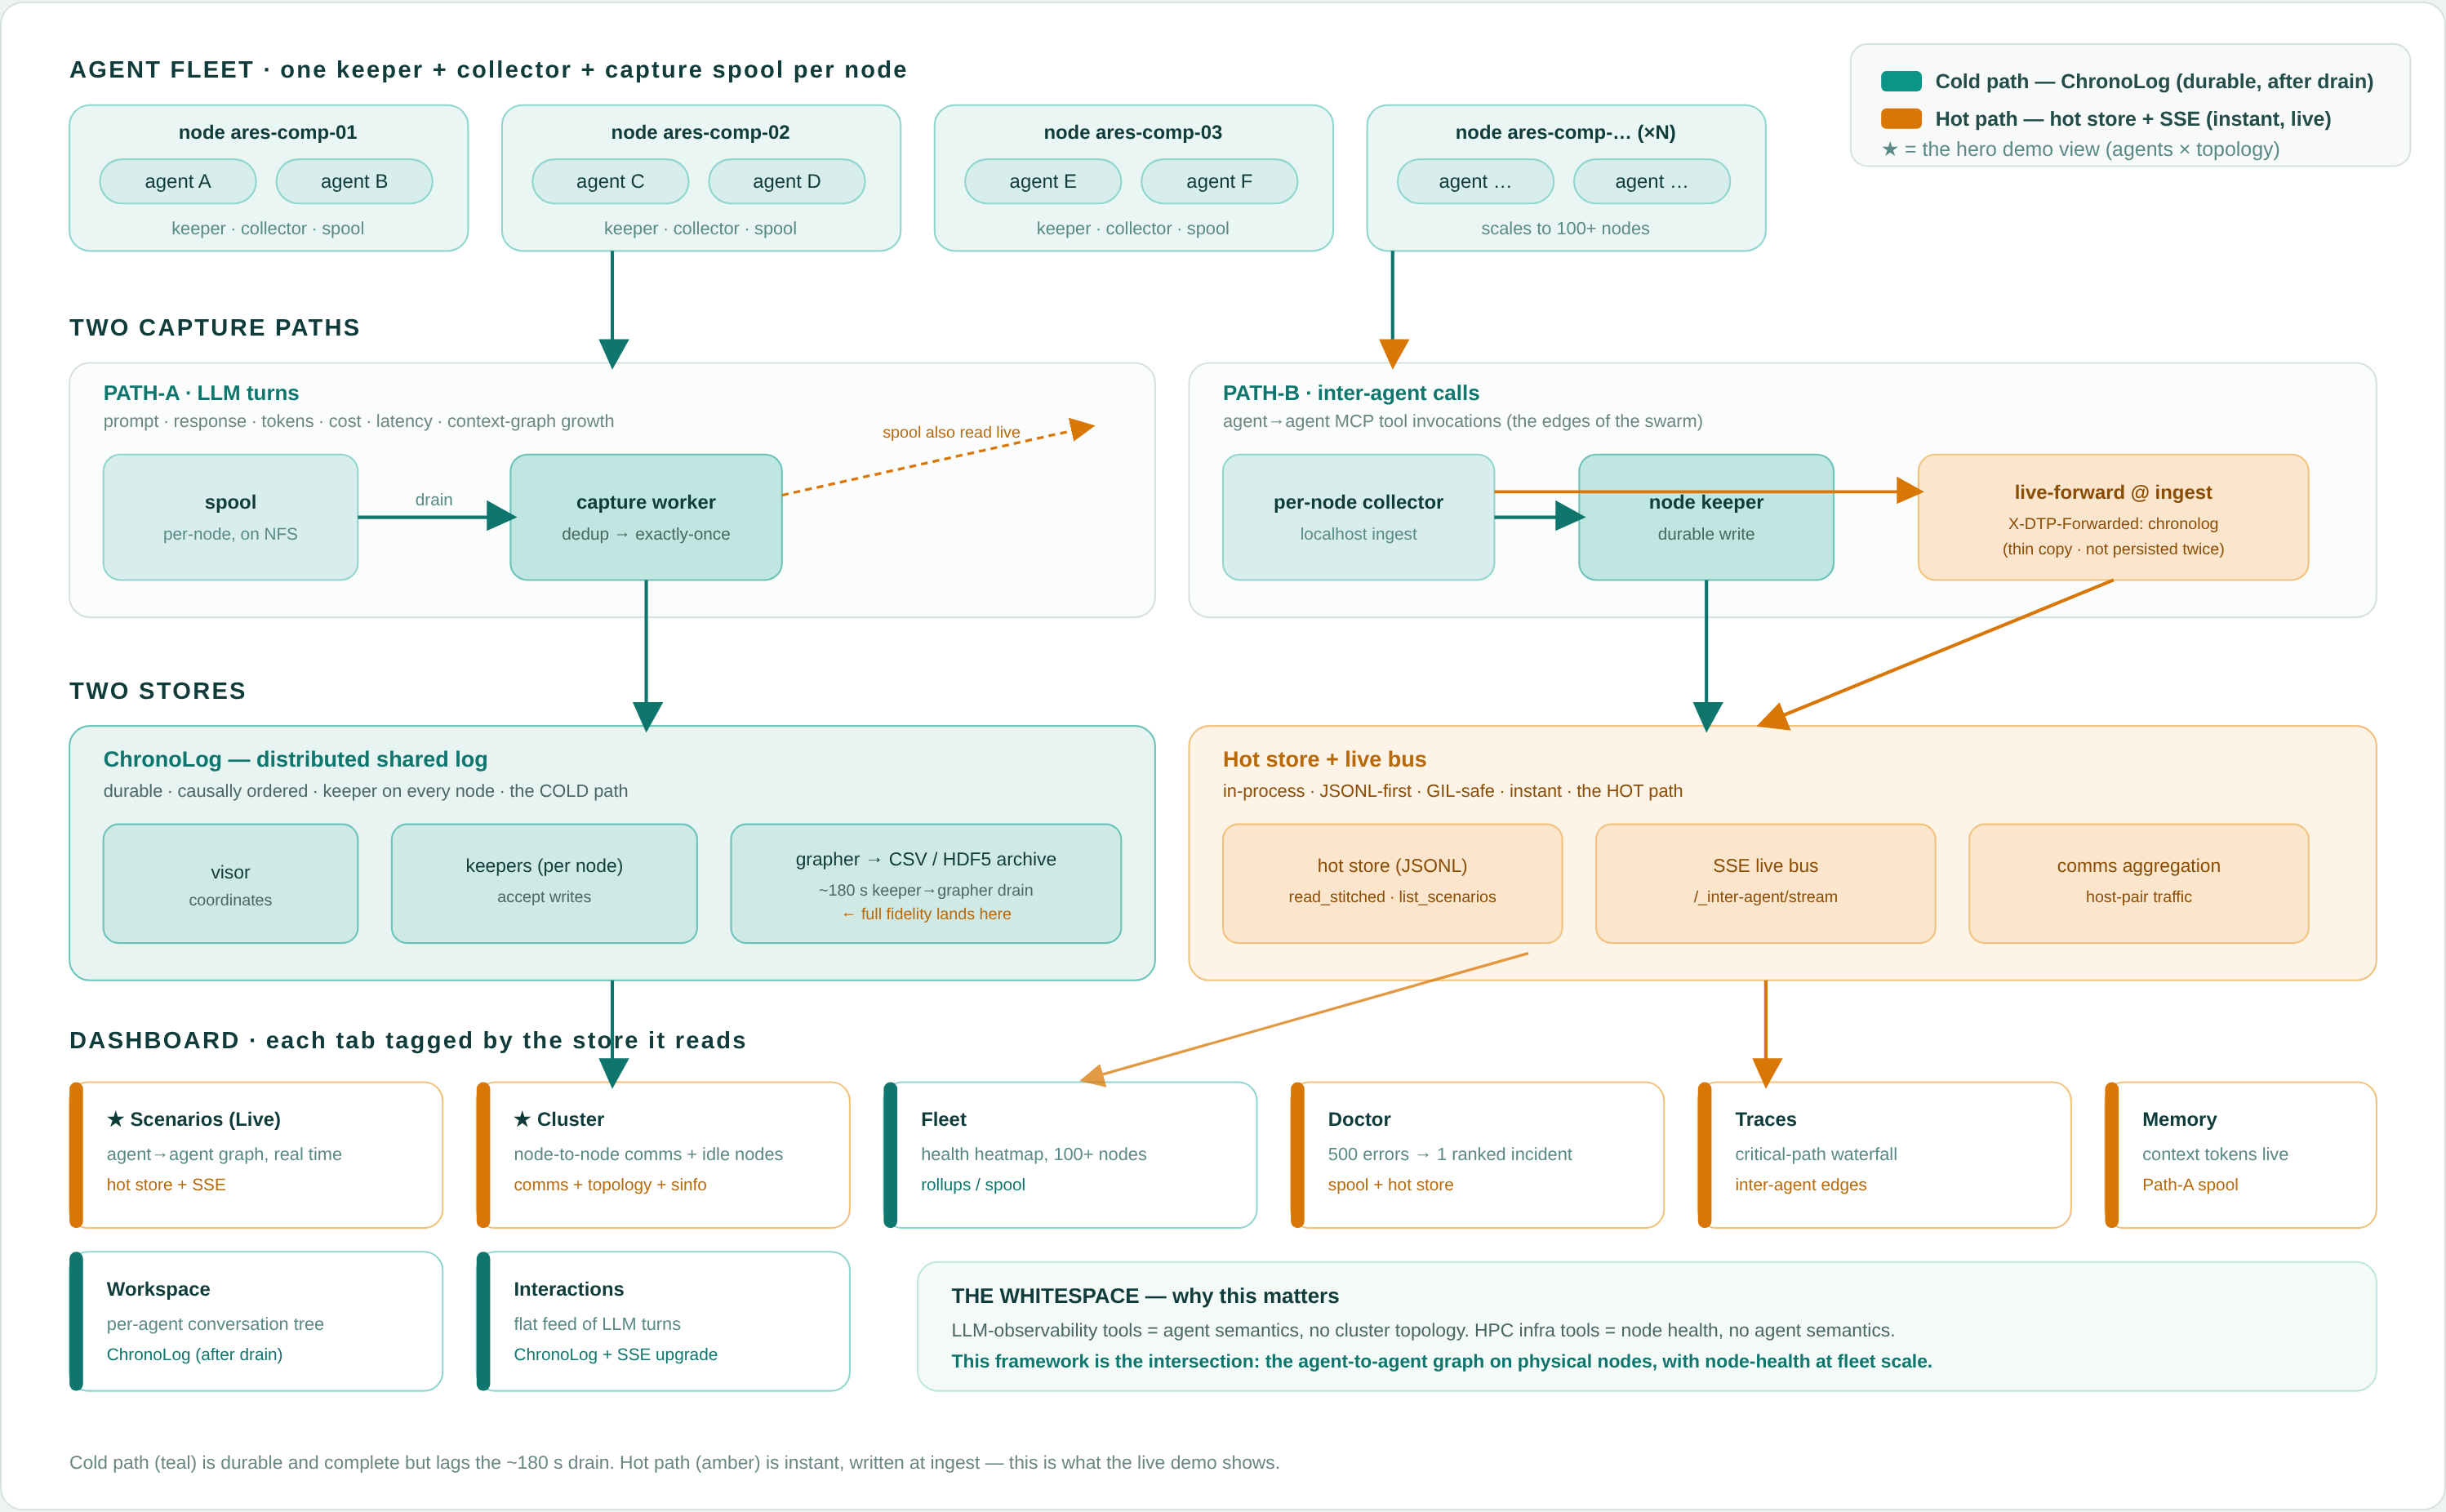
\includegraphics[width=\linewidth]{figures/dataflow}
  \caption{The two-path architecture. Path-A carries LLM turns through a
  node-local spool drained by a capture worker; Path-B carries inter-agent
  calls through a per-node collector. Both persist to ChronoLog through the
  node-local keeper; the dashboard reads ChronoLog (cold, full fidelity)
  and a local hot store (live).}
  \label{fig:dataflow}
\end{figure}

Every datum enters the system through one of two ingest paths
(Figure~\ref{fig:dataflow}), both terminating in ChronoLog via the keeper on
the producing node.

\textbf{Path-A} carries the intra-agent plane: LLM interactions (one record
per turn), context-graph deltas (one record per working-memory add or
eviction), and recovery events. Producers call a small capture library that
appends the record to a node-local, append-only \emph{spool}; a separate
\emph{capture worker} process periodically drains the spool into ChronoLog
stories.

\textbf{Path-B} carries the inter-agent plane: agent-to-agent MCP calls. Each
logical call is emitted as a \emph{pair} of events sharing a correlation
identifier: a \texttt{start} when the delegation is issued and a
\texttt{done} when it completes, the latter carrying status and latency. Agents
POST these events to a \emph{collector} daemon on their own node
(\texttt{localhost:5650}); the collector writes them to the node-local
ChronoLog keeper and simultaneously forwards a thin copy to the dashboard,
which feeds the live views (\S\ref{sec:design-read}).

The two paths differ deliberately. Path-A events are large (full prompts and
responses), produced at low rate (one per turn, i.e.\ per LLM call), and
consumed mostly after the fact, so a durable local buffer plus a batch
drain fits. Path-B events are small, structurally fixed, and latency-relevant (the live
scenario graph is drawn from them), and they define the cross-agent causal
structure; a daemon that stamps, persists, and immediately fans
them out is the better match. What the paths share is the destination and the discipline: node-local
append on the producing machine (R5), durable persistence in the log (R3),
and host attribution stamped at source (R1).

The dashboard itself is a \emph{pure reader}: a Flask application serving a
React single-page app that reconstructs every view from ChronoLog and the
hot store, and captures nothing on its own
(\S\ref{sec:design-isolation}).

\section{Mapping Agent Semantics onto the Log}
\label{sec:design-mapping}

ChronoLog organizes data as chronicle $\to$ story $\to$ event
(\S\ref{sec:bg-chronolog-model}). The mapping adopted here
(Table~\ref{tab:schema}) uses chronicles to partition by \emph{data kind}
and stories by \emph{entity}, so that every read pattern of
Chapter~\ref{chap:analytics} replays exactly one story:

\begin{table}[h]
\centering
\small
\begin{tabular}{@{}llll@{}}
\toprule
\textbf{Chronicle} & \textbf{Story} & \textbf{Holds} & \textbf{Path} \\
\midrule
\texttt{llm\_interactions} & \emph{session id} & LLM turns & A \\
\texttt{context\_graphs}   & \emph{session id} & working-memory deltas & A \\
\texttt{recovery\_events}  & \emph{session id} & recovery/backtrack events & A \\
\texttt{ia\_<scenario>}    & \texttt{edges}    & inter-agent \texttt{start}/\texttt{done} events & B \\
\texttt{metrics\_rollup}   & \texttt{minute}   & per-(host, minute) fleet buckets & rollup \\
\texttt{\_\_index\_\_}     & \texttt{scenarios} / \texttt{sessions} & listing index & both \\
\bottomrule
\end{tabular}
\caption{The chronicle/story schema: chronicles partition by data kind,
stories by entity. Session-scoped stories serve the conversation and
memory reads; the per-scenario edge story serves graph and trace reads;
the rollup and index stories are written by the capture side so that
readers never scan.}
\label{tab:schema}
\end{table}

\paragraph{Session identity.} The load-bearing convention is the session
identifier \texttt{role@scenario} (e.g.\ \texttt{writer@scenario-x}). It is
simultaneously the ChronoLog story name for all Path-A data of that agent,
the \texttt{from\_session}/\texttt{to\_session} endpoint on Path-B edges, and
the join key the dashboard uses when a clicked node in the scenario graph
opens that agent's conversation. Scoping the role by scenario keeps the
identifier globally unique across concurrent scenarios while leaving it
human-readable. Because the same string names the spool file, the
ChronoLog story, and the graph node, the identity round-trips through every
tier with no lookup table. This is R1's ``joinable planes'' made concrete:
the join is by construction, not by correlation heuristics.

\paragraph{Causal structure.} Cross-agent causality is carried by two
explicit fields on Path-B events. The \texttt{correlation\_id} stitches the
\texttt{start}/\texttt{done} pair of one call into a single edge; the
optional \texttt{parent\_correlation\_id} records the call being
\emph{serviced} when a new call was issued, giving the tracer exact call
trees. When instrumentation does not propagate the parent, the tracer falls
back to inference from session identity and time nesting
(\S\ref{sec:analytics-tracing}), the Mystery-Machine position on the
spectrum of \S\ref{sec:bg-tracing-lineage}, with explicit propagation as the
Dapper position when available. Within a session, Path-A records carry a
monotonic per-stream \texttt{sequence\_id}, which orders turns without
reference to wall clocks.

\paragraph{Listing without enumeration.} One practical gap in the substrate
is the absence of a chronicle-enumeration operation in the client binding:
there is no way to ask ``which scenarios exist?'' without knowing their
names. The design routes around it with an \texttt{\_\_index\_\_} chronicle:
every component that first sees a new scenario or session appends a one-line
event (\texttt{\{"v": <name>\}}) to a well-known index story, and listing
becomes a replay of that story, deduplicated in first-seen order. The index
is append-only and idempotent to re-add, so it needs no coordination among
the writers. The pattern is a small instance of the log-as-substrate principle: when a
query is missing, materialize it as another log.

\section{Write Path and Delivery Semantics}
\label{sec:design-write}

The write path is engineered backwards from R5 (never perturb the agent) and
R3 (never lose, never duplicate).

\paragraph{The spool as write-ahead buffer.} A Path-A producer's fast path is
an append of one JSON line to a per-\((\text{session}, \text{kind})\) spool
file, opened with \texttt{O\_APPEND} so that concurrent writers interleave
atomically at line granularity. No network, no lock, no dependency on any
downstream component being alive: if ChronoLog, the capture worker, or the
dashboard is down, agents keep running and the spool absorbs the backlog.
The capture library injects and guarantees exactly three fields:
\texttt{session\_id}, a monotonic \texttt{sequence\_id} (seeded from the
maximum found on disk, so monotonicity survives producer restarts), and a
\texttt{timestamp}. It treats the rest of the record as an opaque
producer contract.

\paragraph{Effectively exactly-once ingest.} The capture worker drains the
spool into ChronoLog on a polling interval. Transport is at-least-once by
construction (after a crash the worker re-reads spool files it may have
partially drained), so ingest must deduplicate. The worker keeps a
\emph{high-water mark} per \((\text{session}, \text{kind})\) stream: the
largest \texttt{sequence\_id} already written to ChronoLog. Only records
above the mark are appended. The critical property is where that state
lives: on startup the worker \emph{rebuilds the marks from ChronoLog
itself}, replaying each session's stories to find the highest sequence
present. The log is thus the single source of truth for what has been
ingested, and the worker carries no durable state of its own. No worker
crash, restart, or migration to another node can cause loss (the spool
retains everything) or duplication (the rebuilt marks skip everything
already present). Records without a natural sequence (recovery events) carry
a unique blob identifier and are deduplicated by set membership, seeded the
same way. The arrangement is the textbook recipe of \S\ref{sec:bg-delivery}
(at-least-once transport plus idempotent, monotonic ingest), instantiated
with the log as its own ledger.

\paragraph{Path-B: persist once per backend.} The collector gives Path-B
events the same guarantees with one extra subtlety. Every event travels to
\emph{two} places: the node-local keeper (durable) and the dashboard (for
the live bus). Naively this double-writes. The design makes the forward
explicit: when, and only when, the collector has successfully written an
event to ChronoLog, it sets a header (\texttt{X-DTP-Forwarded: chronolog})
on the forwarded copy. The dashboard honors the header by preserving the
collector-stamped identifiers verbatim and skipping its own ChronoLog write,
storing only the hot copy. If the keeper write failed, the collector
forwards \emph{without} the header and the dashboard persists the event
through its own backend; the placement is degraded, but the event is
not lost. The net
contract: each event is persisted exactly once per backend, and the
identifiers (\texttt{event\_id}, timestamps) are identical in both copies,
so the live view and the durable view never disagree about identity.

\paragraph{Graceful degradation.} One more fallback closes the path: an
agent's \texttt{emit()} tries the node-local collector first and falls back
to POSTing directly to the dashboard's ingest endpoint if the collector is
down. The fallback sends no forwarded header, so the dashboard persists
normally. An agent therefore observes at most a failed local HTTP call
before falling back: never a lost edge, and never back-pressure from the
log (R5).

\section{The Read Problem: Hot and Cold Paths}
\label{sec:design-read}

Writing to an ingest-optimized log is easy; reading it live is the hard
part. As established in \S\ref{sec:bg-chronolog-design}, freshly appended
events sit inside the keeper$\to$grapher acceptance window
(20--30\,s measured end-to-end in the deployments used here) before they
are readable from the archive. Worse, a replay the player cannot
answer does not return stale data but \emph{blocks} for the client's
${\sim}180$\,s query timeout, in a Python client that holds the GIL
throughout. A dashboard
that naively replayed stories on request would freeze for minutes precisely
while the fleet is live, a direct violation of R2.

The design response is a lambda-style split (\S\ref{sec:bg-log}) with the
acceptance window as the boundary:

\paragraph{The cold path} is ChronoLog itself: complete, durable, ordered,
and authoritative, but late. Full-fidelity views (a session's complete
conversation, post-hoc analysis) read it, either by live replay once a story
has drained or from the grapher's archive files. Reads that risk touching
un-drained state are avoided structurally: the listing index of
\S\ref{sec:design-mapping} is read \emph{archive-first}, because a live
replay against a never-written index story blocks indefinitely
(\S\ref{sec:design-isolation}). The evaluation later hardened this rule
into a deployment mode: after live replay proved unreliable end-to-end
on the cluster, archive-first reading was generalized from
the listing index to \emph{every} replay the serving processes issue,
bounding staleness at the drain window
(\S\ref{sec:eval-freshness}, \S\ref{sec:eval-limitations}).

\paragraph{The hot path} serves R2 and is populated \emph{at the moment of
ingest}, before ChronoLog acceptance. It has two elements. First, a
\emph{hot store}: the ingest endpoint appends every Path-B event to a local
JSONL file per scenario, and all live read APIs (the scenario graph, the
node-communication view, fleet aggregation, the tracer) read this store,
an instant, append-only local read that can never block on the log. Second,
a \emph{live bus}: an in-process publish/subscribe fan-out that pushes each
newly ingested event to server-sent-event subscribers, so the browser
renders edges as they happen rather than polling. Path-A has the analogous
arrangement: the Health view and the per-agent memory panels read the
capture spool directly (the spool doubling as Path-A's hot store)
while ChronoLog remains the durable copy.

\paragraph{The late-join protocol.} A client that opens a live stream
mid-run needs history plus continuity without gaps or duplicates. The bus
protocol delivers the stored backlog first, then live frames, and the
subscription is registered \emph{before} the backlog is read, so an
event ingested during the handoff appears in both, and the client
deduplicates by event identifier. Delivery to subscribers is intentionally
weaker than delivery to storage: per-subscriber queues are bounded and drop
oldest under pressure, and a publish never blocks or raises into the ingest
path. By the time an event reaches the bus it is already durable, so the
live stream is a best-effort projection of a reliable log, not a second
reliability domain (R5).

\paragraph{Consistency model.} Each view advertises, in effect, one of two
freshness classes: hot views are eventually consistent with the log but
fresh to within the ingest latency (measured in
Chapter~\ref{chap:evaluation}); cold views are complete and ordered but
stale up to the acceptance window. Because both are projections of the same
event stream with identical identifiers
(\S\ref{sec:design-write}), the classes converge: after the drain, a hot
view's content is a prefix-complete subset of the cold view's, and the
operator can always escalate from ``live picture now'' to ``authoritative
record later'' without changing tools.

\section{Process and Failure Isolation}
\label{sec:design-isolation}

The deployment decomposes into single-responsibility processes per node
(agents, collector, capture worker), plus one dashboard for the
allocation. Three isolation rules, each learned from a concrete failure on
live clusters, govern the decomposition.

\paragraph{The dashboard is a pure reader.} An early configuration ran the
capture worker as a thread inside the dashboard process. On startup the
worker warms its high-water marks by replaying sessions
(\S\ref{sec:design-write}); on a cluster where a story sat inside the
acceptance window, that replay blocked while holding the GIL, and the Flask
server never finished binding its port. The lesson generalizes: a process
that must always answer (the dashboard) may never share an interpreter with
a component that may legitimately block on remote state (the capture
worker). They now run as separate processes, and the rule extends to reads:
no request handler ever issues a replay that could touch un-drained state.

\paragraph{Never block on state that may not exist.} A fresh cluster
exhibits a boundary case. Replaying an index story that has \emph{never
been written} blocks indefinitely: there is no data to drain, and none
will ever arrive. Listing reads are therefore archive-first (the archive's
absence is detectable instantly, while a live replay's futility is not),
with live replay behind an explicit opt-in; and a brand-new deployment
seeds the index with a one-shot append-only sync pass, sidestepping the
blocking warm-up entirely.

\paragraph{Normalize identity at the edge.} Host names arrive from multiple
authorities (reverse DNS reports \texttt{ares-comp-3}, SLURM reports
\texttt{ares-comp-03}), and any view that joins on host names (fleet
health, the cluster graph, allocation membership) silently drops nodes if
the two spellings coexist. All host names are therefore canonicalized (digit
padding stripped) at every boundary where they enter a data structure.
Identity normalization, like time, belongs at the edge of the system, not
in each consumer.

Failure containment follows from the decomposition: an agent crash loses
nothing already spooled or emitted; a collector crash falls agents back to
direct dashboard ingest; a capture-worker crash pauses draining while the
spool absorbs; a dashboard crash affects only observation (capture
continues); and a ChronoLog outage degrades the system to hot-store-only
operation, with the spool and collector queues replaying into the log when
it returns.

\section{Extensibility: Adapters and Capabilities}
\label{sec:design-adapters}

Every dashboard view is declared as a \emph{capability} (conversations,
scenarios, diagnostics, fleet, tracing, \dots) served by a \emph{source
adapter}, an interface discovered at runtime through a Python
entry-point group. The shipped ChronoLog adapter serves all capabilities;
at startup the application discovers active adapters, mounts only the API
blueprints some adapter can serve, and advertises the active set to the
frontend, which renders only those tabs. The seam exists for third parties:
a deployment with a different substrate implements the adapter interface
and gains the dashboard unchanged. The same seam is what
makes the offline demo mode (local stores, no cluster) a configuration
rather than a fork. This chapter's design is thereby separable: the capture
paths, delivery semantics, and hot/cold split of
\S\S\ref{sec:design-write}--\ref{sec:design-read} are ChronoLog-specific
engineering; the analytics of Chapter~\ref{chap:analytics} depend only on
the capability interface.
